
\chapter{Architecture Research} \label{sec:architectureresearch}

The literature review also identified a variety of modelling techniques, including Steady-state modelling, Dynamic Modelling, Surrogate Modelling, and Optimisation. 

The Ahuora Digital Twin Platform is currently built to support only steady state modelling. However, to explore the potential for integrating more advanced live data processing techniques, the IDAES Process Systems Engineering Framework was employed as a testbed.

The IDAES framework is a Python library that provides tools for modelling and simulating chemical processes. It is designed to be extensible, allowing for the addition of new modelling techniques.

Using the IDAES framework, experimentation with live data processing techniques was conducted. This testing aimed to evaluate the feasibility of integrating these advanced techniques into the Ahuora Digital Twin Platform. By leveraging IDAES, the platform can be designed to support the incorporation of more sophisticated modelling techniques in the future.

\section{Research Questions}

The research investigation aimed to answer the following questions:

\begin{itemize}
    \item \textit{RQ1:} How does the Ahuora Simulation Platform need to be modified to support dynamic modelling, surrogate modelling, and optimisation?
    \item \textit{RQ2:} What architecture would best support the integration of live data processing techniques into the Ahuora Digital Twin Platform?
\end{itemize}

\textit{RQ1} focuses on future needs and long-term vision. This is important to help minimise the amount of rework required when implementing new features. \textit{RQ2} focuses on the immediate needs of the project, and is important for developing a pilot implementation.

\section{Dynamic Modelling} 

I used the IDAES framework to develop a dynamic model of a steam tank, with a valve controlling the inlet and outlet pressure and flow rate. A PID controller was used to control the valve opening fraction to regulate the pressure in the tank.

\begin{figure}
    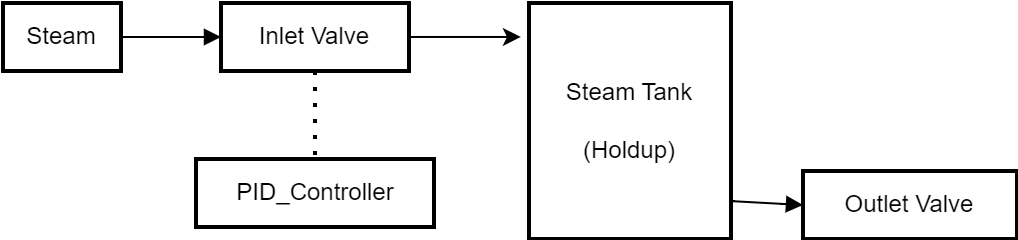
\includegraphics[width=0.9\textwidth]{dynamicmodelling.png}
    \caption{Dynamic Modelling of a Steam Tank}
    \label{fig:dynamicmodelling}
\end{figure}

This provided a simple example of a dynamic system. The inlet and outlet valve and the PID controller were not dynamic models: From a mathematical perspective, this means their properties were fully determined by the inlet and outlet conditions. The only dynamic model was the Steam Tank. From a mathematical perspective, this means that the state of the steam tank was determined by the inlet and outlet conditions, but also the previous state of the tank, i.e how ``full" the tank is.


\section{Key Findings}\label{sec:dynamicmodelling}

\begin{itemize}
    \item The IDAES framework is well-suited to dynamic modelling, as it provides tools for creating and solving differential equations. It can easily model the same system at different time scales.
    \item The Ahuora Simulation Platform will require substantial changes to support dynamic modelling. Rather than storing a single value for each property, it will need to store the state of each property at each time step.
    \item This will also require significant UI changes to view the state of the system at different time steps. This could be achieved through some sort of time slider, and graph visualisations of properties over time.
    \item Specifying the initial conditions of the system will be more complex, as the user will need to specify the initial state of dynamic properties, such as the initial tank level. Other properties, such as the valve opening fraction, will need to be specified as functions of time.
\end{itemize}

\section{Surrogate Modelling}
Surrogate Modelling is the process of creating a simplified model of a complex system. This is usually done using machine learning techniques. This provides a good test case of implementing data-driven modelling techniques in the IDAES framework.

IDAES includes a framework for data-driven modelling called PySMO. This provides utilities for training polynomial, Radial Basis Function, and Kriging models to approximate the behaviour.

% TODO: Explain how we tested surrogate modelling in IDAES (perhaps just from the research article)

\subsection{Key Findings}\label{sec:surrogatemodelling}

Surrogate Modelling may be achieved using IDAES's built-in PySMO libraries, or other similar libraries such as OMLT. It is reasonably straightforward to train a surrogate model to represent a non-dynamic unit operation, but dynamic unit operations get significantly more complex - instead of modelling a single value, the surrogate model must be able to model the entire time system. There are some methods of doing this, such as using neural ODEs, Residual Networks, Operator Networks, or some other sort of convolutional network. There is little research into applying these methods in the field of chemical and process simulation, especially in the context of mathematical modelling such as the IDAES framework.

The exact same process for surrogate modelling can also be used to model unit operations from historical data. This is useful when there is no mathematical model of the unit operation, but there is historical data available. This would be very useful when applying the Ahuora Digital Twin Platform to existing factories, where the exact mathematical properties of the unit operations are unknown but there is a wealth of historical data available. Online Learning techniques could be used to update the surrogate model in real-time, as new data becomes available. This is a key step in turning a ``simulation" into a ``digital twin", as it allows the model actively adapt to real-world conditions.

Because of the limited functionality of the Ahuora Digital Twin Platform, it is currently beyond the scope of this project to implement a surrogate model. However, the IDAES framework is well-suited to this task, and it is likely that a surrogate model could be implemented in the future.

Additionally, the Ahuora Digital Twin Platform will need a user interface to support creating these different types of models. As surrogate modelling is a complex process, the user interface will need to be able to guide the user through the process of creating a surrogate model from a dataset, and provide feedback on the quality of the model. This will require a significant amount of work, and will likely be a key focus of future development.


\section{Optimisation and Control}

%TODO: Add an explanation about how we tested optimisation and control in IDAES


\subsection{Key Findings} \label{sec:optimisationcontrol}

Implementing Model Predictive Control in IDAES is relatively straightforward, as long as there is a dynamic model of the system, a cost function, and the optimisation problem is well-posed. The Ahuora Digital Twin Platform does not support optimisation yet, but this will be supported in the future.

IDAES's Caprese library can simulate model predictive control, but in order for it to truly be useful IDAES needs to be paired with a real-time data processing system. The real-time data processing system will need to be able to make the controlling actions suggested by the MPC in real-time, and then inform the MPC of the system's response. This requires integration with the industry-specific SCADA systems that are used to control factories.

This project will focus on the data-gathering and processing aspects of this problem, rather than the control aspects. However, suggestions on how to implement control will be provided.



The research in the literature review and the experimentation in IDAES provided a good understanding of the requirements for the Ahuora Digital Twin Platform. The next step was to develop a architecture for the platform that would support these requirements. A pilot implementation was then developed to demonstrate the feasibility of the architecture.

\section{Research Conclusions} \label{sec:researchconclusions}

The current Ahuora Simulation Platform is split into three main parts:

\begin{itemize}
    \item The Frontend UI, which is written in Typescript/React and runs in the user's web browser. This is responsible for rendering the flowsheet, and allowing the user to interact with the simulation.
    \item The Backend API, which is written in Python/Django and runs on the server. This is responsible for storing the simulation data, orchestrating calls to run the simulation, and returning the results to the user.
    \item The IDAES solving engine, which is written in Python and runs on the server. This is responsible for solving the simulation, and returning the results to the API. It has been seperated out from the API to allow it to be scaled independently.
\end{itemize}

Over time, the Ahuora Simulation platform will be expanded to support dynamic modelling, surrogate modelling, and optimisation.

Additionally, there are also a number of other tools that are used in industry for collecting and processing sensor data. There may be an integrated solution or a number of different tools that are used together, but they can be grouped by their functionality:
\begin{itemize}
    \item Data Collection: These tools are responsible for collecting data from sensors and storing it in a database. They may also provide tools for cleaning and preprocessing the data. This includes IoT networks and SCADA systems.
    \item Data Processing: These tools are responsible for processing the data to extract useful information. This may include machine learning models, statistical analysis, or other data processing techniques. Generally, these tools will sit within some sort of framework or pipeline, such as Apache Kafka, Flink, or a custom solution.
    \item Data Storage: These tools are responsible for storing the data in a way that is accessible to the other tools. This may include databases, data lakes, or other storage solutions. In Model-Based Systems Engineering, this is often referred to as a Knowledge Base.
\end{itemize}

\begin{figure}
    \centering
    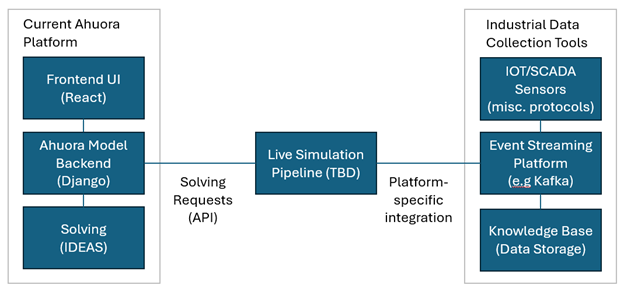
\includegraphics[width=0.9\textwidth]{architecture.png}
    \caption{Anticipated method of implementing the Ahuora Simulation Platform into an industrial system.}
    \label{fig:architecture}
\end{figure}

 Thus, the Ahuora Simulation platform will need to be connected to these tools to access the sensor data. However, there is a discrepancy in the use cases of the Ahuora Simulation Platform and the standard industrial stack. The Ahuora Simulation Platform is designed with experimentation and analysis in mind, which are usually offline\footnote{Many use cases of the Ahuora Simulation platform include designing new factories or modifications to a factory. These tasks mostly use historical data, and are a distinctly seperate problem from live prediction and control.} tasks performed by expert engineers. The standard industrial stack is designed for real-time prediction and control, which are online tasks performed by operators. Both the engineer's workflow and the operator's workflow will require all the modelling and simulation techniques identified, but the operator's workflow will use a fixed set of models.

\begin{table}[ht]
    \centering
    \caption{Comparison of Engineer's and Operator's Requirements}
    \begin{tabular}{|c|p{0.35\textwidth}|p{0.4\textwidth}|}
        \hline
        \textbf{Requirement} & \textbf{Engineer} & \textbf{Operator} \\
        \hline
        Use Case & Design, Retrofit, & Maintenance, Monitoring, Control \\
        \hline
        Modelling & Creates and modifies multiple models & Fixed set of models, only certain parameters may change\\
        \hline
        Data Usage & Historical data, likely preprocessed or cleaned & Real-time raw data \\
        \hline
        Reliability & It is acceptable if incorrectly configured models don't solve & Model must be correct; Requires 100\% reliability \\
        \hline
    \end{tabular}
    \label{tab:requirements}
\end{table}

Because of the different use cases, while the Ahuora Simulation platform needs to be designed so that it is easy to design and build a model, this functionality will not be required in operation. The model could be considered ``frozen'' at this point, where only certain parameters can be changed based on the real-time data. It does not make sense to expose functionality to edit the model to an operator. 



Deploying the a model in production would likely only be done by a trained engineer who manages the plants' SCADA systems.
The deployment would have to be custom for each plant, depending on the SCADA system in use, the sensors available, and the model being used. 
Making a User Interface for this process would be very challenging, and would limit support to only a certain number of protocols. 
Thus, it can be considered that the interface, pipeline, or service between the Ahuora Simulation Platform and the SCADA system is a custom software component. 
In the Proposed Architecture (\Cref{sec:proposed_architecture}), this is referred to as the Digital Twin Adapter. It represents a framework, API, or service that serves as a bridge between the simulation platform and the SCADA system. 

